% SpecMol -- KDD 2027 D&B ACM (acmart) version. AUTO-built from main.tex by build_acm.py.
% Camera-ready TODO: remove nonacm/anonymous, add \acmConference + CCS + keywords;
% re-balance main vs \appendix per author preference.
\documentclass[sigconf,nonacm,anonymous,review]{acmart}
\settopmatter{printccs=false,printacmref=false}
\let\Bbbk\relax  % avoid clash between amssymb and acmart's newtxmath
\usepackage{amssymb}
\usepackage{pifont}
\newcommand{\cmark}{\textcolor{green!55!black}{\checkmark}}
\newcommand{\xmark}{\textcolor{red!70!black}{\ding{55}}}
\setcopyright{none}
\renewcommand\footnotetextcopyrightpermission[1]{}

\begin{document}
\title{[Experiment, Analysis, and Benchmark] When Does Geometry-Aware Pretraining Help? A Matched-Protocol Map Separating Finetuned-Encoder Gains from Inert Frozen 3D Injection in Molecular Property Prediction}
\author{Anonymous Author(s)}
\affiliation{\institution{Anonymous Institution}\country{}}

\begin{abstract}
Pretrained 3D molecular encoders are reused downstream in two very different ways: cheaply, by injecting their frozen pair/geometry features into a 2D model, or expensively, by end-to-end finetuning---yet whether either route beats a strong fingerprint baseline, and which, is rarely settled under one matched protocol. We deliver \textsc{Fire} (\emph{Frozen-feature Injection Reusability Evaluation}), a named, reusable, domain-general diagnostic that asks whether a \emph{frozen, pretrained feature} fed to a downstream model contributes \emph{signal} or merely \emph{parameters}, and a controlled map of molecular property prediction that results from applying it. \textsc{Fire} packages three controls---individually known, but here combined and validated end-to-end: a shape-matched \textbf{random-pair null} that replaces the pretrained pair tensor with same-shape noise at the consumption site, isolating geometry from added parameters; a \textbf{frozen-probe$\rightarrow$finetune absolute correction} that prevents an under-trained linear probe from mis-ranking encoders; and a \textbf{matched-split descriptor random-forest (RF) ceiling} that quantifies fingerprint saturation on the exact test fold. Instrumenting a single spectral pipeline (a ChebNet~II backbone consuming Uni-Mol pair representations) with these controls across six MoleculeNet endpoints and quantum stress tests, we find a clean two-regime separation. A real end-to-end \emph{Uni-Mol} finetune---on the same matched split as the baselines---draws the regime line cleanly: it beats the matched RF on FreeSolv ($0.435$ vs.\ $0.720$ standardized RMSE) and Lipophilicity ($0.521$ vs.\ $0.643$) and ties it on BBBP ($0.826$ vs.\ $0.814$) and ClinTox ($0.832$ vs.\ $0.812$), while a descriptor RF still leads the genuinely saturated BACE ($0.906$ vs.\ $0.859$), ESOL, and composition-dominated QM7. This recovery is a \emph{finetuning} effect, not a frozen-injection one: a frozen Uni-Mol probe scores far worse (ClinTox $0.488$, below random; Lipophilicity $0.794$ RMSE), and every frozen 3D-injection variant (static gate, pair-biased attention, atom--pair co-update) ties its shape-matched random-pair null and the 2D baseline on every cell---including a true B3LYP/6-31G(2df,p)-DFT-coordinate QM9 dipole stress test, where a charge-aware RF still leads ($0.845$ vs.\ best deep $0.880$). The gain is the finetuned encoder's capacity, not the injected geometry. We release a fully regenerable harness. Regression RMSE is on standardized labels and is not comparable to the kcal/mol literature; the saturation thesis is bounded to BACE/ESOL/QM7.
\end{abstract}

\maketitle

\section{Introduction}
\label{sec:intro}

Molecular property prediction is a central problem in drug discovery and computational chemistry, and a long line of work has shown that accurate predictions hinge on representations that capture both the topology of chemical bonds and the geometry of three-dimensional conformers. Two-dimensional graph neural networks exploit bond-level structure but cannot directly access through-space interactions such as steric clashes, hydrogen bonds, or favorable stacking. Conversely, purely three-dimensional models depend on the quality of conformer generation and tend to be computationally expensive at the scale of high-throughput screening. A practical alternative is to start from a strong two-dimensional backbone and inject three-dimensional information only where it is most useful, but the design space for such an injection remains underexplored.

Self-supervised pretraining has produced increasingly capable molecular encoders along both modalities. On the two-dimensional side, contrastive frameworks such as MolCLR \citep{wang2022molclr} and graph transformers such as GROVER \citep{rong2020grover} learn transferable atom and bond representations from millions of unlabeled molecules. On the three-dimensional side, Uni-Mol \citep{zhou2023unimol} pretrains an SE(3)-equivariant encoder over conformer ensembles and produces, in addition to atomic embeddings, a dense pair representation $P \in \mathbb{R}^{N \times N \times d_p}$ that encodes geometric relationships between every atom pair. Multi-view pretraining approaches such as GraphMVP \citep{liu2022graphmvp} have further shown that aligning two- and three-dimensional views during pretraining benefits downstream prediction. The complementary question of how to consume a frozen three-dimensional pair representation at downstream time, without retraining the upstream encoder, has received considerably less attention.

Spectral graph neural networks offer a particularly clean entry point for such an injection. The recently introduced ChebNet II \citep{he2022chebnetii} parametrizes graph convolutions as Chebyshev polynomials of the symmetric normalized Laplacian and admits per-edge weights as a first-class input. This makes the edge weights of the Laplacian a natural locus at which to fold in three-dimensional information: an off-the-shelf pair representation can be projected to a scalar gate on each chemical bond, and the resulting weighted Laplacian then drives the spectral filtering. The challenge is that naively initializing such a gate to small or random values immediately perturbs the spectrum away from the unweighted baseline, destabilizing the contrastive pretraining objective and erasing the inductive bias of the two-dimensional backbone before any useful learning has taken place.

We study this injection problem empirically rather than proposing a single new method. Two mechanisms, both built on the same backbone---a dual-path Chebyshev~II encoder with low-pass and high-pass towers, fused with a fingerprint MLP and pretrained by an NT-Xent contrastive loss across four views---serve as the subjects of study, differing only in how the frozen pair representation enters the spectral filter. The first, \textbf{V2-T5}, applies a small MLP followed by a symmetrized sigmoid with bias initialization $b{=}{+}5$ to the Uni-Mol pair representation, yielding an initial per-bond gate of approximately $0.993$; this near-identity initialization preserves the two-dimensional baseline at epoch zero and lets the gate move away from one only when the gradient supports it. The second, \textbf{T7}, stacks a higher-capacity pair-biased multi-head attention block on top of this gate, with a per-head sigmoid that is itself initialized near the residual identity. Against both we run a strict V0 (2D-only) control on the same split, seeds, and budget, together with a fingerprint-only control and a 30-seed random forest, because such classical controls are frequently omitted from molecular benchmarks yet turn out to be highly competitive.

To compare the variants fairly we adopt the Uni-Mol scaffold-fold split with matched seeds, training budget, and reporting format within each benchmark (all cells at three training seeds $\{9, 19, 29\}$). Two regimes emerge. On the \emph{non-saturated} endpoints, deep models---once properly finetuned rather than read out by an under-trained frozen probe---are competitive with or beat the matched classical baselines: a finetuned V0 (the 2D encoder; $n{=}3$ init seeds, single fold-0, \S\ref{sec:finetune-correction}) reaches BBBP $0.860$ and FreeSolv $0.602$ RMSE, beating the matched RF ($0.814$ / $0.720$), and at nine frozen-probe seeds the deep variants already sit at BBBP $0.828$--$0.831$, tying the matched RF ($0.814$) and above the $30$-seed Deng2023 forest ($0.799$, a different split protocol). On the \emph{fingerprint-saturated} endpoints the map says use the descriptor model: on BACE the matched RF reaches $0.906$ AUC and exceeds every deep variant by roughly $14$ points, and likewise dominates ESOL (\S\ref{sec:crossN})---a ceiling no graph-side change in our study penetrates, which we read as marking where a cheap descriptor is the right tool; Lipophilicity and ClinTox are boundary cases that our own end-to-end Uni-Mol finetune resolves into the non-saturated regime---it beats or ties the matched RF there (\S\ref{sec:finetune-correction}). What does \emph{not} move the metric, in either regime, is the cheap frozen 3D injection itself: every injected variant ties its shape-matched random-pair null and the 2D baseline, and on FreeSolv---the endpoint where a 3D-pair effect is most often reported---it is the geometry-free V0 ($0.647 \pm 0.029$ RMSE, $n{=}9$) that is nominally \emph{ahead} of the 3D-injected V2-T5 ($0.673 \pm 0.065$), a within-variance tie that does not lean toward geometry. The one mechanism that looked promising---an aromatic-routing gate on the three audited BBBP seeds (Pearson with the aromatic-bond indicator in $[0.6,0.7]$)---did \emph{not} replicate when six further seeds were audited, so we do not advance it as a finding (\S\ref{sec:ablations}); T7's attention gate, meanwhile, stays in a near-identity-residual regime across every audited checkpoint. The positive, then, is the finetuned encoder's capacity, not the injected geometry. A forensic featurization audit (\S\ref{sec:featurization-control}) further shows how easily an \emph{unmatched} control can manufacture an apparent gain---a silent unidirectional-bond bug in our own loader shifted apparent V2-T5 BACE performance by several AUC points.

\paragraph{\textsc{Fire}: a named, reusable diagnostic for frozen-feature injection.}
We package the three controls into a single, reusable diagnostic we call
\textsc{Fire} (\emph{Frozen-feature Injection Reusability Evaluation}), and
this packaged, validated protocol---not any of its individual ingredients---is
the methodological object we contribute. \textsc{Fire} answers one question
that recurs far beyond chemistry: when a downstream model ingests a
\emph{frozen, pretrained feature}, does that feature contribute \emph{signal},
or merely \emph{parameters}? It does so with three steps run \emph{without
retraining the upstream encoder}: (i)~a shape-matched \textbf{random-pair Null}
that swaps the frozen feature for same-shape noise at the consumption site, so
any apparent gain is attributed to the data rather than to the added capacity
and wiring; (ii)~a \textbf{frozen-probe$\rightarrow$Finetune absolute
correction} that prevents an under-trained linear probe from mis-ranking
encoders (here it silently re-ranks by up to $\sim$$0.1$~AUC and reads ClinTox
\emph{below random}); and (iii)~a \textbf{matched-split descriptor-RF Ceiling}
on the \emph{exact} test fold, which says whether any deep model---injected or
finetuned---can clear a strong classical baseline at all. Each ingredient is
individually known---shuffled/permutation nulls, linear-probe-vs-finetune
diagnostics, and the strong-classical-baseline critique each have ample
precedent (\S\ref{sec:related})---so we claim novelty for none of them in
isolation. What is new is their \emph{combination} into a falsifiable,
drop-in protocol, its \emph{validation} on a single matched pipeline, and the
\emph{when}-map it yields; and that \textsc{Fire} is \emph{domain-general}---the
frozen feature is a 3D pair embedding here, but it is equally a learned table
embedding, a foundation-model representation, or any precomputed descriptor, so
\textsc{Fire} applies to any frozen-feature injection pipeline with molecular 3D
injection as the running case study. Its application yields a \emph{positive,
actionable} verdict---properly finetuned geometry-aware encoders are the right
tool on the non-saturated endpoints, whereas cheap frozen injection is not---
rather than a bare negative result.

\paragraph{Contributions.}
\begin{itemize}
\item \textbf{(C1) A \textsc{when}-does-it-help map for downstream reuse of pretrained 3D encoders.} Under one matched scaffold-fold protocol we sort six MoleculeNet endpoints into a fingerprint-\emph{saturated} regime, where a descriptor Random Forest matches or beats every deep model (BACE, ESOL, and composition-dominated QM7), and a \emph{non-saturated} regime, where a properly end-to-end finetuned encoder is competitive with or beats RF (BBBP, FreeSolv, ClinTox, and Lipophilicity---the last two confirmed non-saturated by a real Uni-Mol finetune that beats or ties the matched RF, \S\ref{sec:finetune-correction}). The map is a falsifiable, reusable diagnostic, not a leaderboard entry.

\item \textbf{(C2) A frozen-probe$\rightarrow$finetune absolute correction that is the source of the positive result.} A frozen ``pretrained embedding $+$ classical head'' evaluation badly under-ranks encoders---the frozen Uni-Mol$+$RF probe scores ClinTox $0.488$ (below random) and BACE $0.722$ (vs.\ matched RF $0.906$)---whereas the \emph{same 2D encoder}, properly finetuned ($n{=}3$ init seeds, single fold-0), becomes competitive with RF on the non-saturated half (V0 BACE $0.758\!\rightarrow\!0.822\!\rightarrow\!0.886$, approaching the matched RF $0.906$; BBBP $0.860$ and FreeSolv beating the matched RF; \S\ref{sec:finetune-correction}). We quantify the probe-vs-finetune gap, provide a drop-in protocol fix, and release an end-to-end Uni-Mol finetune runner as the protocol-correct replacement for the frozen probe.

\item \textbf{(C3) A shape-matched random-pair null that attributes the gain to the encoder, not the injected geometry.} Across a static edge gate (V2-T5), pair-biased attention (T7), and an atom$\leftrightarrow$pair co-update (T8), the real pretrained pair never separates from a same-shape noise tensor within seed variance on any cell, including a true B3LYP-DFT-coordinate QM9 dipole stress test (RF $0.845$ vs.\ best deep $0.880$ on the identical subset); a gate-movement probe shows this null is data-bound, not a wiring artifact (\S\ref{sec:dft}). The finetuned-encoder competitiveness of C1--C2 therefore comes from capacity, while cheap frozen 3D injection contributes no usable signal.

\item \textbf{(C4) A regenerable evaluation harness and an honesty-bounded baseline panel.} Every reported cell regenerates from released per-seed JSON via a single \texttt{paper/make\_tables.py}; we release the random-pair null, split reconstruction, matched classical baselines (RF, Chemprop, frozen-Uni-Mol-embedding), the end-to-end Uni-Mol finetune runner, and a forensic featurization audit (a one-line loader bug manufactures a $7.4$-AUC swing) as first-class artifacts, with regression reported on standardized labels and the saturation thesis explicitly bounded. Beyond the molecular case study, two of these artifacts are transferable, citable methodological findings in their own right: a forensic featurization audit showing that a single silent unidirectional-bond loader bug manufactures a $7.4$-AUC swing---larger than the entire deep-vs-classical gap on BACE---cross-checked against fourteen widely cited public repositories (\S\ref{sec:featurization-control}), and a frozen-probe$\rightarrow$finetune correction that converts an apparently uncompetitive encoder (ClinTox $0.488$, below random) into a competitive one (\S\ref{sec:finetune-correction}); both are warnings any frozen-feature benchmark---chemical or otherwise---can adopt directly.
\end{itemize}

Two further analyses are reported with their caveats in the body rather than headlined: a chemically interpretable but initialization-sensitive aromatic-routing pattern in the trained V2-T5 gate that holds on the audited $n{=}3$ BBBP cohort but does \emph{not} replicate at $n{=}9$ (\S\ref{sec:ablations}); and a forensic audit of a unidirectional-bond featurization regression in our own loader~\cite{nguyen2021graphdta}---which alone shifts apparent V2-T5 BACE performance by $7.4$ AUC points---cross-checked against fourteen widely cited public repositories (\S\ref{sec:featurization-control}) and offered as a cautionary reproducibility note. The higher-capacity T7 and T8 variants, whose pair-biased attention and co-update machinery carry no novelty over prior transformers, are reported only as controlled explorations in results and limitations.

% ---------------------------------------------------------------------
\section{Related Work}
\label{sec:related}

\paragraph{Downstream injection of frozen, pretrained 3D geometry.}
Closest to our setting are models that try to obtain geometry's benefit without
3D coordinates at inference. \texttt{SCAGE} \citep{qiao2025scage} pretrains a
2D+3D multi-task encoder with distance-masked attention and a fingerprint
objective on five million MMFF conformers and then fine-tunes 2D-only
(BACE~0.854, BBBP~0.734); it \emph{trains through} the very frozen-injection
regime we isolate, but never freezes the 3D source at inference, never shuffles
the pair as a control, and never separates frozen-probe from fine-tuning---so it
cannot tell whether the geometry signal survives downstream injection or is, as
we find, recovered only by fine-tuning. \texttt{3D-PGT} \citep{wang2023threedpgt}
distills bond-length/angle/dihedral geometry \emph{into the weights} during
generative pretraining and discards 3D at test time (BACE~0.809); we instead
keep a frozen pair tensor and inject it at inference, and we add the random-pair
null that 3D-PGT lacks. The pair-as-attention-bias mechanism our T7 rung uses is
itself not new: \texttt{Graphormer} \citep{ying2021graphormer} adds
shortest-path/edge encodings as additive attention bias (2D, from scratch),
\texttt{MAT} \citep{maziarka2020mat} adds a \emph{trainable} inter-atomic
distance matrix as bias (end-to-end, no external 3D encoder; BBBP~0.728,
FreeSolv~0.263), and \texttt{EGT} \citep{hussain2022egt} maintains gated
all-pairs $N\times N$ edge channels updated end-to-end. T7/T8 therefore carry
\emph{no attention novelty}; our only departure is the \emph{source}
(a frozen Uni-Mol pair rather than a learned-from-scratch bias), the
\emph{target} (a spectral backbone), and the \emph{null protocol} none of these
works run. \texttt{KA-GNN} \citep{li2025kagnn} similarly already adds 5\,\AA{}
through-space ``contact'' edges to a molecular GNN (BACE~0.890$\approx$RF,
BBBP~0.787, no pretraining), so the analogous contact-edge rung we report is a
completeness control and a null demonstration, not a contribution.

\paragraph{Critical audits of molecular benchmarks and the utility of 3D.}
A skeptical literature, which our study extends rather than overturns, questions how much modern molecular models actually gain over classical baselines. On the benchmark side, \citet{deng2023systematic} train tens of thousands of models and find a Random Forest on RDKit-2D/Morgan descriptors best on BACE, BBBP, ESOL, and Lipophilicity; \citet{xia2023whydeep} argue more bluntly that deep models often cannot beat fingerprint-plus-tree baselines, and the concurrent benchmark of \citet{praski2025embedding} reaches the same conclusion against pretrained encoders \emph{including} Uni-Mol. The activity-cliff stress test of \citet{vantilborg2022cliffs} and the demonstration that scaffold splits overestimate virtual-screening performance \citep{guo2024scaffold} further temper reported gains. Our fingerprint-saturation result (C2) deliberately \emph{replicates} this pattern under a matched Uni-Mol scaffold-fold protocol rather than claiming it anew; what is new is that the saturation persists \emph{through} a frozen 3D-pair injection path. On the geometry side, \citet{hamakawa2025conformation} run the closest negative control to ours, retraining Uni-Mol on deliberately wrong conformers: tellingly, their geometry channel \emph{is} used---wrong conformers degrade accuracy---on quantum-mechanical targets under \emph{fine-tuning}, whereas we find a \emph{frozen} pair representation injected into a 2D spectral backbone inert, and tied by a pair-shuffled random control, on fingerprint-saturated MoleculeNet endpoints. The contrast (frozen injection vs.\ native fine-tuning; saturated ADMET/physchem vs.\ geometry-rich quantum targets) delimits \emph{where} a cheap downstream 3D injection can be expected to help, and motivates the controls we adopt.

\paragraph{What the closest works do not do.}
The three \textsc{Fire} controls each have precedent, but no prior work runs all
three together on a \emph{frozen-feature injection} pipeline, which is precisely
what lets us separate injected-geometry \emph{signal} from added
\emph{parameters} and from a saturated benchmark.
Table~\ref{tab:positioning} makes the gap legible. Benchmark audits establish
the RF ceiling but never inject or null a frozen feature
\citep{deng2023systematic,xia2023whydeep,praski2025embedding,wu2018moleculenet};
representation-probing work compares frozen-vs-finetuned \emph{rankings} but not
the absolute correction, and never isolates frozen-feature signal from
parameters via a shape-matched null \citep{wang2023molgrapheval,sun2022gnnpretrain};
and the geometry-pretraining line shows 3D helps \emph{under finetuning} but
trains \emph{through} the frozen-injection regime we isolate, never freezing the
3D source at inference, never shuffling the pair as a control, and never
separating frozen-probe from finetune
\citep{zhou2023unimol,qiao2025scage,wang2023threedpgt,hamakawa2025conformation}.
We are, to our knowledge, the first to \emph{package and validate} the three
controls jointly and report the resulting \textsc{when}-map.

\begin{table}[t]
\centering
\caption{What the closest works do \emph{not} do. Columns are the three
\textsc{Fire} controls plus the frozen-injection setting they presuppose.
\cmark{} = the work performs that control/setting; \xmark{} = it does not.
Each control is individually known; the contribution is that no prior work
combines all four on a frozen-feature injection pipeline.}
\label{tab:positioning}
\small
\setlength{\tabcolsep}{4pt}
\begin{tabular}{@{}lcccc@{}}
\toprule
 & Frozen & Shuffled & Probe$\to$FT & Matched-RF \\
Work (representative) & inject & null & correction & ceiling \\
\midrule
Deng2023~\cite{deng2023systematic}        & \xmark & \xmark & \xmark & \cmark \\
MolGraphEval~\cite{wang2023molgrapheval}  & \xmark & \xmark & \xmark$^{\dagger}$ & \xmark \\
MoleculeNet~\cite{wu2018moleculenet}      & \xmark & \xmark & \xmark & \xmark \\
Uni-Mol~\cite{zhou2023unimol}             & \xmark & \xmark & \xmark & \xmark \\
SCAGE~\cite{qiao2025scage}                & \xmark$^{\ddagger}$ & \xmark & \xmark & \xmark \\
3D-PGT~\cite{wang2023threedpgt}           & \xmark$^{\ddagger}$ & \xmark & \xmark & \xmark \\
Hamakawa2025~\cite{hamakawa2025conformation} & \xmark & \cmark$^{\S}$ & \xmark & \xmark \\
\midrule
\textbf{\textsc{Fire} (ours)}             & \cmark & \cmark & \cmark & \cmark \\
\bottomrule
\end{tabular}
\par\smallskip
{\footnotesize $^{\dagger}$Compares frozen-vs-finetune \emph{rank} correlation,
not the absolute mis-ranking we correct. $^{\ddagger}$Trains \emph{through}
geometry then finetunes 2D-only; never freezes the 3D source at inference.
$^{\S}$Perturbs conformers under \emph{finetuning} (a wrong-geometry control),
not a shape-matched shuffle at a frozen-injection site.}
\end{table}

\paragraph{The SOTA ceiling we do not contest.}
Recent supervised and pretrained models post far higher leaderboard scores than our audit targets: MoLFormer-XL~\cite{ross2022molformer} reaches BBBP~$0.937$ and ClinTox~$0.948$; the 3D-space-modeling SpaceFormer~\cite{lu2025spaceformer} reaches BACE~$0.966$ (GEM~\cite{fang2022gem}~$0.985$); and equivariant geometry models such as Equiformer~\cite{liao2023equiformer} reach QM9 dipole MAE~$\sim$$0.011$~D. We cite these as the upper envelope, not a target: our contribution is a matched-protocol map of \emph{when} a finetuned geometry-aware encoder helps over a strong classical baseline, not a leaderboard entry. Crucially these numbers are not mutually comparable---canonical Uni-Mol scores BBBP~$0.729$ under its own scaffold split but $0.907$ under a cleaned out-of-distribution split~\cite{lu2025spaceformer}, a $>$$0.17$ AUC swing from split and de-duplication alone that exceeds most model-vs-model gaps. This split-sensitivity is itself part of our argument that single-split leaderboard AUC is not a robust axis for the question we ask.

\section{Method}
\label{sec:method}

\subsection{Notation}
Let $G=(\mathcal{V},\mathcal{E})$ be a molecular graph with $N=|\mathcal{V}|$ heavy atoms and chemical bonds $\mathcal{E}\subseteq\mathcal{V}\times\mathcal{V}$. Each atom carries a feature vector $\mathbf{x}_i\in\mathbb{R}^{d_x}$ (atomic number, degree, hybridization, etc.); each bond an edge attribute $\mathbf{e}_{ij}\in\mathbb{R}^{d_e}$. We additionally consume a frozen pair representation $\mathbf{P}\in\mathbb{R}^{N\times N\times d_p}$ produced by a pretrained Uni-Mol encoder \citep{zhou2023unimol}, indexed over all atom pairs $(i,j)$. The chemical-bond adjacency $A\in\{0,1\}^{N\times N}$ is symmetric (each bond contributes both directed edges $(i,j)$ and $(j,i)$) and induces the symmetric normalized Laplacian $L_{\mathrm{sym}}=I-D^{-1/2}AD^{-1/2}$, where $D$ is the degree matrix.

\subsection{Backbone: Dual-Path Chebyshev Spectral GNN}
Our backbone, denoted \texttt{LH\_Direct}, processes $G$ along two parallel spectral paths and fuses them with a molecular fingerprint stream. Each spectral path is a Chebyshev~II encoder \citep{he2022chebnetii} that applies an order-$K$ polynomial filter to the normalized Laplacian:
\begin{equation}
    h^{(\ell)} = \sum_{k=0}^{K} \theta_k\, T_k(\tilde L)\, h^{(\ell-1)},
    \qquad \tilde L = 2L_{\mathrm{sym}}/\lambda_{\max} - I,
    \label{eq:chebnetii}
\end{equation}
where $T_k$ is the $k$-th Chebyshev polynomial and the coefficients $\{\theta_k\}_{k=0}^{K}$ are learnable. We fix $\lambda_{\max}{=}2$ for $\tilde L$ to avoid per-batch eigenvalue estimation. The two paths use independent coefficients tuned, by construction, towards low-pass and high-pass behavior respectively. The pooled graph representations $h_l, h_h\in\mathbb{R}^{d_h}$ are concatenated with a fingerprint embedding $h_{\mathrm{fp}}=\mathrm{MLP}(\mathrm{FP}(G))$, where $\mathrm{FP}$ concatenates PubChem (881), MACCS (167), and ErG (441) fingerprints into a $1489$-dimensional vector. The fused representation $z = [h_l; h_h; h_{\mathrm{fp}}]$ is the only object exposed to the downstream head.

\subsection{Variant V0: Two-Dimensional Baseline}
The V0 baseline runs \texttt{LH\_Direct} with $A$ unchanged, i.e.\ all bonds carry equal Laplacian weight. V0 ignores the Uni-Mol pair representation entirely and serves as the strict two-dimensional reference.

\subsection{Variant V2-T5: Static Pair-to-Edge Gating}
\label{sec:v2t5}
V2-T5 augments V0 with a learnable scalar gate on each chemical bond, computed from the frozen Uni-Mol pair representation. Concretely, for each bond $(i,j)\in\mathcal{E}$ we form
\begin{equation}
    g_{ij} = \sigma\!\left( \tfrac{1}{2}\bigl(\mathrm{MLP}_\phi(\mathbf{P}_{ij}) + \mathrm{MLP}_\phi(\mathbf{P}_{ji})\bigr) + b \right),
    \label{eq:v2t5gate}
\end{equation}
where $\mathrm{MLP}_\phi$ is a two-layer scalar-output network shared across edges, the symmetrization ensures $g_{ij}=g_{ji}$, and $\sigma$ is the logistic sigmoid. Crucially we initialize the bias term $b=+5$, which gives an initial gate of $\sigma(5)\approx 0.993$ across all bonds. This near-identity initialization preserves the V0 dynamics at epoch zero, so the contrastive pretraining objective starts from a near-optimal point and is free to move $g_{ij}$ away from $1$ only when gradient signal justifies it. The reweighted Laplacian $L_{\mathrm{sym}}(g)$ is then plugged into Eq.~(\ref{eq:chebnetii}) in place of $L_{\mathrm{sym}}$.

\subsection{Variant T7: Pair-Biased Attention with Per-Head Gating}
\label{sec:t7}
T7 stacks a four-head pair-biased attention block on top of the V2-T5 gate. Each head computes pair-biased attention $\mathrm{softmax}(QK^\top/\sqrt{d_h} + \mathbf{P})\,V$ over the node features, and---following ReZero~\cite{bachlechner2021rezero} and LayerScale~\cite{touvron2021cait}---each head's output is scaled by a learnable per-head gate $\sigma(\gamma_h)$ before the residual sum, with $\gamma_h\in\mathbb{R}$ initialized to $-2$ (so $\sigma({-}2)\approx 0.119$). T7 is the only mechanism we study with an explicitly gated attention output, so its closed-gate dynamics are directly observable from the trained $\sigma(\gamma_h)$ histogram (\S\ref{sec:experiments}). We treat T7 as a higher-capacity comparison point for V2-T5 rather than a proposed method: it lets us ask what a more expressive injection path actually learns under the same contrastive objective.

\subsection{Training Objective and Downstream Evaluation}
\label{sec:training}
\paragraph{Self-supervised pretraining.} All variants are pretrained with a four-view NT-Xent contrastive objective that pulls together low-pass, high-pass, mixed, and fingerprint embeddings of the same molecule and pushes apart embeddings of different molecules within a batch. We use temperature $\tau{=}0.5$, batch size $512$, and early-stopping based on training loss with patience $100$ epochs.

\paragraph{Downstream linear probe.} After pretraining, the encoder is frozen and a two-layer logistic regression head (with a single Dropout layer set to $p{=}0.2$ during training and disabled during evaluation) is trained on top of the fused representation $z$. For each pretraining seed we run three independent evaluation restarts with probe-init seeds $\{9,19,29\}$ and report the test metric at the validation-best epoch. To prevent early-epoch noise from locking model selection on a lucky-spike checkpoint, we require both a minimum of $200$ probe epochs before any selection update and a strict improvement tolerance of $10^{-4}$.

% ---------------------------------------------------------------------
\section{Experiments}
\label{sec:experiments}

\subsection{Setup}
\paragraph{Datasets.} Six MoleculeNet-derived benchmarks: BBBP (binary classification, 2{,}039 molecules), BACE (1{,}513), and ClinTox (1{,}478, two tasks) for classification; FreeSolv (regression, 642), ESOL (1{,}128), and Lipo (4{,}200). All use the Uni-Mol scaffold-fold split protocol (\S\ref{sec:featurization-control}); the regression benchmarks use a fixed train/valid/test assignment under the same seed. Tox21 (7{,}831 molecules, 12 tasks) was intended but its all-pairs Uni-Mol pair extraction exceeded our memory budget and is deferred (\S\ref{sec:discussion}).
\paragraph{Seeds and budget.} We use three training seeds $\{9,19,29\}$ for contrastive pretraining across all cells, matching the three-seed protocol of the Uni-Mol scaffold-fold pipeline. Each pretrained checkpoint is evaluated over three downstream restarts (probe seeds $\{9,19,29\}$), collapsed to a per-training-seed mean before the table standard deviation. Pretraining runs up to $1000$ epochs (batch $512$, NT-Xent $\tau{=}0.5$, early-stop on training loss with patience $100$; all reported runs reach $\ge 970$). The probe runs to a fixed budget (500 epochs for classification, 2000 for regression) with the validation-best checkpoint chosen after a $200$-epoch warm-up; the selected epoch lies well below the budget for every run.
\paragraph{Baselines.} V0 (2D-only); FP-only (fingerprint MLP head, no graph encoder); a 300-tree Random Forest on Morgan~$+$~11 RDKit-2D descriptors (the Deng2023 descriptor recipe~\citep{deng2023systematic}, 30 restarts), evaluated on the model's \emph{exact} test split; the Chemprop D-MPNN~\cite{yang2019chemprop} on the same split; a frozen Uni-Mol molecular-embedding~$+$~RF control---the ``Uni-Mol-emb$+$RF (frozen probe)'' row---that consumes Uni-Mol's representation directly rather than through the spectral gate, isolating whether any inertness is a property of the benchmark or of our injection; and, where available, a matched end-to-end \emph{Uni-Mol finetune} via the released runner (the ``Uni-Mol (FT)'' row, \S\ref{sec:finetune-correction})---the same encoder's own supervised number on the identical split, kept distinct from the frozen probe so the crippled probe is never read as finetuned Uni-Mol. The RF and Chemprop baselines fold the deep model's validation split into training (neither needs a held-out validation fold) but are scored on the \emph{identical} test fold; on all three regression benchmarks every molecule yields a valid 3D conformer ($0$ failures across the $642/1{,}128/4{,}200$ FreeSolv/ESOL/Lipo molecules), so the matched RF and deep models are evaluated on exactly the same test set.
\paragraph{Compute and hyperparameters.} Each pretraining run uses a single NVIDIA RTX 5000 Ada (32~GB) at $\approx$four hours per (variant, seed); the probe runs in under an hour. No hyperparameters are tuned per variant: all inherit $K{=}10$, $d_h{=}512$, dropout $0.2$, and the V0 optimizer and scheduler. Code, processed datasets, and the post-B4 rebuild scripts are released (\S\ref{sec:reproducibility}).

\subsection{Main Results}
Table~\ref{tab:whenmap} collapses all eight endpoints into a single matched-protocol \textsc{when}-map: it reads off, for each task, whether a descriptor random forest or a finetuned geometry-aware encoder is the right tool, and shows that the cheap frozen 3D injection (the ``best deep'' column) wins neither regime. We use it as the navigation key for the per-table results that follow.

\begin{table*}[t]
\centering
\caption{\textbf{When does each tool win? A matched-protocol regime map.}
All cells are on the \emph{identical} scaffold-fold split, so columns are
directly comparable. Classification is AUC ($\uparrow$); regression is
\emph{standardized} RMSE ($\downarrow$, not kcal/mol); QM7 is MAE ($\downarrow$).
The per-row winner is in \textbf{bold}. Two regimes emerge: on
\emph{saturated} endpoints a plain descriptor random forest is unbeaten, while
on \emph{non-saturated} endpoints a properly finetuned geometry-aware encoder
(off-the-shelf Uni-Mol) wins or ties. The cheap \emph{frozen} 3D
injection (best deep variant) is inert in \emph{both} regimes---it never
separates from V0 or its shape-matched random-pair null. $\dagger$: MolTrain
exposes no seed control, so this Uni-Mol~(FT) cell is a deterministic
single-split internal-5-fold-CV point estimate (std${\approx}0$ is \emph{not} a
zero-variance claim); only BBBP/ClinTox~(FT) carry real $n{=}3$ variance.
QM7/QM9-$\mu$ have no frozen-probe/FT cell (---); their ``best deep'' is the
strongest 3D arm on the same molecules. Ties within seed variance are noted in
the regime column. Sources: Tables~\ref{tab:classification}--\ref{tab:dft}.}
\label{tab:whenmap}
\small
\setlength{\tabcolsep}{5pt}
\begin{tabular}{@{}llcccccl@{}}
\toprule
Endpoint & Metric & Matched & Frozen Uni-Mol & Uni-Mol & Best deep & Regime & Recommended \\
 &  & RF & $+$RF probe & (FT) & (variant) &  & tool \\
\midrule
BBBP    & AUC $\uparrow$  & $0.814$          & $0.765$ & $0.826^{\dagger}{\scriptstyle\pm.008}$ & $\mathbf{0.831}$ {\scriptsize(V2\text{-}T5)} & Non-sat.\ (FT\,$\approx$\,deep\,$\geq$\,RF) & finetuned encoder \\
BACE    & AUC $\uparrow$  & $\mathbf{0.906}$ & $0.722$ & $0.859^{\dagger}$                       & $0.763$ {\scriptsize(V2\text{-}T5)}          & \textbf{Saturated} (RF wins)               & descriptor RF \\
ClinTox & mAUC $\uparrow$ & $0.812$          & $0.488$ & $\mathbf{0.832}{\scriptstyle\pm.043}$ & $0.829$ {\scriptsize(V2\text{-}T5)} & Non-sat.\,/\,boundary (FT\,$\approx$\,deep\,$\approx$\,RF) & finetuned encoder \\
FreeSolv& RMSE $\downarrow$& $0.720$         & $0.683$ & $\mathbf{0.435}^{\dagger}$              & $0.647$ {\scriptsize(V0)}                    & Non-sat.\ (FT/deep\,$<$\,RF)                & finetuned encoder \\
ESOL    & RMSE $\downarrow$& $\mathbf{0.361}$& $0.580$ & $0.395^{\dagger}$                       & $0.771$ {\scriptsize(V2\text{-}T5)}          & \textbf{Saturated} (RF wins)               & descriptor RF \\
Lipo    & RMSE $\downarrow$& $0.643$         & $0.794$ & $\mathbf{0.521}^{\dagger}$              & $0.873$ {\scriptsize(V2\text{-}T5)}          & Non-sat.\,/\,boundary (FT\,$<$\,RF)         & finetuned encoder \\
\midrule
QM7      & MAE $\downarrow$ & $\mathbf{\sim\!99}$ & --- & --- & $137\text{--}149$ {\scriptsize(deep)}           & \textbf{Saturated} (composition-dom.)      & descriptor RF \\
QM9-$\mu$& RMSE $\downarrow$ & $\mathbf{0.845}$    & --- & --- & $0.880$ {\scriptsize(V0, DFT geom.)}            & Geometry-pure, RF still leads              & descriptor RF \\
\bottomrule
\end{tabular}
\end{table*}
% Auto-generated by paper/make_tables.py -- do not edit by hand.
\begin{table}[t]
\centering
\caption{Classification test AUC, mean $\pm$ sample std over per-seed means under matched Uni-Mol scaffold-fold split. BBBP 2D-Only/SEG use $n{=}9$ training seeds; BBBP PBA and BACE/ClinTox deep cells use $n{=}3$; RF is a Morgan$+$RDKit-2D random forest (the descriptor recipe of \citet{deng2023systematic}, 30 restarts) recomputed on the model's \emph{exact} test split. ClinTox cells report macro-averaged AUC across its two constituent tasks. The ``Uni-Mol-emb$+$RF'' row is a frozen Uni-Mol embedding with an RF head (a probe, \emph{not} Uni-Mol's own performance). ``Uni-Mol (FT)'' is the end-to-end finetuned Uni-Mol on the identical split (MolTrain exposes no seed control: cells with std${\approx}0.000$ are deterministic single-split internal-5-fold-CV point estimates, \emph{not} a zero-variance claim; only BBBP and ClinTox showed seed variance). The two ``$\pm$'' semantics differ: deep-variant cells (2D-Only/SEG/PBA) report \emph{seed} variance, whereas Uni-Mol~(FT) cells report training-set-resampling sensitivity (internal 5-fold CV), so the two columns' error bars are not directly comparable.}
\label{tab:classification}
\begin{tabular}{lccc}
\toprule
Variant & BBBP & BACE & ClinTox \\
\midrule
2D-Only & 0.828 $\pm$ 0.027 & 0.757 $\pm$ 0.047 & 0.804 $\pm$ 0.046 \\
FP-only & -- & 0.846 $\pm$ 0.012 & -- \\
RF & 0.814 $\pm$ 0.008 & 0.906 $\pm$ 0.003 & 0.812 $\pm$ 0.039 \\
Chemprop & 0.815 $\pm$ 0.008 & 0.862 $\pm$ 0.010 & 0.975 $\pm$ 0.004 \\
Uni-Mol-emb$+$RF & 0.765 $\pm$ 0.008 & 0.722 $\pm$ 0.012 & 0.488 $\pm$ 0.027 \\
Uni-Mol (FT) & 0.826 $\pm$ 0.008 & 0.859 $\pm$ 0.000 & 0.832 $\pm$ 0.043 \\
SEG & 0.831 $\pm$ 0.032 & 0.763 $\pm$ 0.010 & 0.829 $\pm$ 0.085 \\
PBA & 0.821 $\pm$ 0.011 & 0.780 $\pm$ 0.027 & -- \\
\bottomrule
\end{tabular}
\end{table}

% Auto-generated by paper/make_tables.py -- do not edit by hand.
\begin{table}[t]
\centering
\caption{Regression test RMSE (lower is better; mean $\pm$ sample std over per-seed means under matched scaffold splits). FreeSolv 2D-Only/SEG use $n{=}9$ seeds; ESOL/Lipo deep cells and PBA use $n{=}3$; RF is a Morgan$+$RDKit-2D random forest (Deng2023 recipe, 30 restarts) on the model's \emph{exact} test fold. all SEG cells (FreeSolv/ESOL/Lipo) use Uni-Mol pair representations; the FreeSolv PBA cell alone uses an RDKit-GBF pair surrogate (\S\ref{sec:v2t5}). RMSE is on the standardized label scale (std${\approx}1$ for all three regression sets; FreeSolv is thus not in kcal/mol---its raw scale is $\sigma{\approx}3.8$ kcal/mol, so a standardized RMSE of $0.7$ is ${\approx}2.7$ kcal/mol and is not comparable to the kcal/mol literature). The ``Uni-Mol-emb$+$RF'' row is the frozen-embedding probe. ``Uni-Mol (FT)'' is the end-to-end Uni-Mol finetune; its std${\approx}0.000$ cells are deterministic single-split internal-5-fold-CV point estimates (MolTrain has no seed control), not a zero-variance claim. The two ``$\pm$'' semantics differ: deep-variant cells (2D-Only/SEG/PBA) report \emph{seed} variance, whereas Uni-Mol~(FT) cells report training-set-resampling sensitivity (internal 5-fold CV), so the two columns' error bars are not directly comparable.}
\label{tab:regression}
\begin{tabular}{lccc}
\toprule
Variant & FreeSolv (RMSE) & ESOL (RMSE) & Lipo (RMSE) \\
\midrule
2D-Only & 0.647 $\pm$ 0.029 & 0.784 $\pm$ 0.104 & 0.874 $\pm$ 0.009 \\
RF & 0.720 $\pm$ 0.007 & 0.361 $\pm$ 0.002 & 0.643 $\pm$ 0.002 \\
Chemprop & 0.879 $\pm$ 0.085 & -- & -- \\
Uni-Mol-emb$+$RF & 0.683 $\pm$ 0.008 & 0.580 $\pm$ 0.004 & 0.794 $\pm$ 0.002 \\
Uni-Mol (FT) & 0.435 $\pm$ 0.000 & 0.395 $\pm$ 0.000 & 0.521 $\pm$ 0.000 \\
SEG & 0.673 $\pm$ 0.065 & 0.771 $\pm$ 0.057 & 0.873 $\pm$ 0.008 \\
PBA & 0.687 $\pm$ 0.070 & -- & -- \\
\bottomrule
\end{tabular}
\end{table}

Tables~\ref{tab:classification} and~\ref{tab:regression} summarize performance, and two regimes emerge: on the non-saturated endpoints (BBBP, FreeSolv) the deep models tie or beat the matched classical baselines, whereas on the fingerprint-saturated endpoints (BACE, ESOL, Lipo) a descriptor random forest leads. \emph{Within} the deep family, no \emph{injection} variant separates from the V0 baseline within seed variance---so where deep is competitive, the gain is the architecture and the finetuned encoder, not the frozen 3D signal. Matched-seed paired tests confirm this on every endpoint: BACE (V2-T5 $+0.005$, paired $t{=}0.18$; T7 $+0.023$, $t{=}0.53$, with T7 below V0 on two of three seeds), ClinTox (V2-T5 $+0.025$, $t{=}0.52$), FreeSolv (the 2D V0 is itself ahead by $0.026$ RMSE at $n{=}9$, $t{=}1.03$, \S\ref{sec:crossN}), and BBBP (V2-T5 $+0.003$ AUC at $n{=}9$)---none significant. On BBBP, V0 and V2-T5 sit within seed variance at $n{=}9$ (V0 $0.828 \pm 0.027$, V2-T5 $0.831 \pm 0.032$; the $+0.003$ V2-T5 margin is well inside the per-seed spread); the $n{=}3$ subset that put V2-T5 at $0.862$ was upper-tail sampling and collapses to this tie when the cell is extended to nine seeds. On BACE the deep variants stay at $\sim$$0.76$ (V2-T5 $0.763 \pm 0.010$) while FP-only reaches $0.846 \pm 0.012$ and the matched RF $0.906 \pm 0.003$---a $\sim$$14$-point fingerprint-saturation gap; the matched RF also dominates ESOL ($0.361$ vs.\ deep $0.78$), so no graph-side change in our study closes the classical gap on the genuinely saturated endpoints (BACE, ESOL; Lipophilicity is a boundary case, \S\ref{sec:discussion}). On regression, V2-T5 ties V0 on ESOL ($0.771$ vs.\ $0.784$) and Lipo ($0.873$ vs.\ $0.874$), and on FreeSolv, at $n{=}9$, V2-T5 ($0.673 \pm 0.065$) is nominally \emph{behind} the matched V0 baseline ($0.647 \pm 0.029$) by a small, non-significant $0.026$ RMSE---the 2D baseline, not the 3D-injected variant, is ahead (\S\ref{sec:crossN}). T7, evaluated on BBBP/BACE/FreeSolv, lands at $0.821$/$0.780$/$0.687$---within the same band---with its per-head attention gate fixed in $[0.122,0.124]$ across all nine audited checkpoints, the near-identity-residual regime of ReZero~\citep{bachlechner2021rezero} and LayerScale~\citep{touvron2021cait}; we report it as a controlled exploration. To test whether this inertness reflects a poor \emph{injection} rather than a saturated benchmark, the ``Uni-Mol-emb$+$RF (frozen probe)'' row consumes the frozen Uni-Mol molecular embedding directly (Random Forest head) on the same split. This frozen probe does not reach the ceiling either---Uni-Mol-embedding RMSE is $0.580$/$0.794$ on ESOL/Lipo (vs.\ RF $0.361$/$0.643$) and only $0.488$ AUC on ClinTox (below random)---so the spectral gate's inertness is a property of these benchmarks, not of our injection path; the frozen probe's weakness is itself a measurement artifact that finetuning corrects (\S\ref{sec:finetune-correction}), which is why we report the end-to-end Uni-Mol finetune separately rather than reading this row as Uni-Mol's performance. All Random Forest cells are recomputed on the model's exact split rather than a regenerated one.

\subsection{Ablations}
\label{sec:ablations}
We isolate the design choices and controls of V2-T5 that we found most consequential during development.

\paragraph{(b) Uni-Mol pair vs.\ random pair representation.}
To test whether the V2-T5 gain over V0 reflects geometric information or merely MLP capacity, we replace $\mathbf{P}$ with an isotropic Gaussian tensor of identical shape (gate, bias, and MLP unchanged) and re-run BBBP on the original three matched seeds. The random-pair variant reaches $0.830 \pm 0.017$ overall and loses to V2-T5 on all three seeds (deltas $+0.014, +0.024, +0.059$; mean $+0.032$; $3/3$ wins, one-sided binomial $p{=}0.125$). At $n{=}3$ matched seeds a paired $t$-test ($\alpha{=}0.05$, two-sided) has $\approx$80\% power to detect a real-vs-random AUC gap of $0.076$ or larger (per-seed $\mathrm{SD}_{\mathrm{diff}}{=}0.023$), and the observed $0.032$ gap ($t{=}2.40$, $p{=}0.14$) is below that floor, so the matched-seed $3/3$ win cannot establish an effect larger than $0.076$~AUC and is statistically indistinguishable from zero at this sample size. The Uni-Mol pair therefore carries a small per-seed signal that an isotropic random tensor does not, but this signal sits below the seed-to-seed test-AUC noise floor and neither variant separates from the V0 envelope within seed variance; on BBBP, V2-T5 functions primarily as a structured MLP gate with a measurable but sub-noise-floor geometry contribution.

\paragraph{(c) Cross-$N$ regression: frozen geometry injection is inert; saturation is endpoint-specific.}
\label{sec:crossN}
A frozen 3D pair representation is most often credited on small regression endpoints, so we examine all three regression benchmarks under the matched V0 control. Under the matched V0 control, the apparent FreeSolv ``win'' we first read against an (unmatched) Random Forest baseline ($\approx 0.04$ RMSE) reverses once the cell is extended to nine seeds. At $n{=}9$ it is V0 ($0.647 \pm 0.029$) that nominally edges V2-T5 ($0.673 \pm 0.065$) by $0.026$ RMSE, with V0 lower on six of the nine seeds and a paired $t{=}1.03$ that does not approach significance; the $n{=}3$ ordering that put V2-T5 ahead did not survive the extension. We therefore treat FreeSolv as a within-seed-variance tie---with the 2D baseline, not the 3D-injected variant, nominally ahead---and read it as the absence of a geometry win rather than its presence. Scaling to ESOL ($n{=}1{,}128$) and Lipo ($n{=}4{,}200$) tells the same story from the other direction: V2-T5 ties V0 to within $0.013$ RMSE on ESOL ($0.771$ vs.\ $0.784$) and on Lipo ($0.873$ vs.\ $0.874$). Once V0 is run on the same data at adequate $n$, no regression endpoint shows a geometry win. The matched Random Forest, by contrast, \emph{dominates} our deep variants on the two larger regression benchmarks---ESOL $0.361 \pm 0.002$ and Lipo $0.643 \pm 0.002$ vs.\ the best deep variant's $0.784$ and $0.874$ (within our matched comparison; Lipophilicity is a boundary case where stronger supervised deep models surpass RF, \S\ref{sec:discussion})---mirroring its BACE margin, so within our matched comparison the fingerprint-saturation ceiling spans classification and regression alike; FreeSolv ($n{=}642$, RF $0.720$) is the lone regression endpoint where a deep variant edges the matched RF. Consuming the frozen Uni-Mol embedding directly (Uni-Mol-emb$+$RF row: RMSE $0.580$/$0.794$ on ESOL/Lipo) does not reach the RF ceiling either, indicating the limitation on these saturated endpoints is the benchmark, not the injection path.

\subsection{Finetuning recovers a competitive encoder on the non-saturated subset}
\label{sec:finetune-correction}

The transductive frozen-probe protocol used elsewhere in this paper reports
a low BACE AUC for the 2D-only encoder (V0~$=0.758$). We treat that number
as a \emph{protocol} measurement, not a property of the model, and audit it
directly. All cells in this subsection are $n{=}3$ initialization seeds on a
single fixed Uni-Mol fold-0 split (variance is init-only, not split), so we
attach a power-bound caveat to every comparison and draw only
ordering-robust conclusions; numbers trace to
\texttt{paper/audits/inductive\_sweep\_2026-06-01.json}. The finetuned cells
(detailed in the appendix) are the \emph{2D-only V0} encoder
(single fold-0); the matched end-to-end \emph{Uni-Mol} finetune---on the same
split as every other baseline---is reported at the end of the subsection and
resolves the boundary endpoints (ClinTox, Lipophilicity) into the
non-saturated regime.

\paragraph{The gain is the encoder, not the injected geometry.}
Crucially, the correction does not rescue the 3D-injection claim. Under
finetune, the geometry-injected arms tie the 2D-only and random-pair arms on
every dataset. On BACE the four arms span only $0.013$ AUC
(V0~$0.886$, V2-T5~$0.880$, T7~$0.886$, random~$0.873$), well inside the
$\pm0.014$ seed noise; on BBBP they span $0.021$ (V0~$0.860$, T7~$0.863$,
random~$0.847$, V2-T5~$0.843$); on FreeSolv they span $0.061$ RMSE with V0
nominally best ($0.602$ vs.\ random $0.630$, T7 $0.629$, V2-T5 $0.663$).
This null is not an artifact of test-structure leakage during pretraining:
switching to the inductive ``train''-only split (encoder never sees
valid/test structures) leaves the finetune ranking unchanged and the arms
still tied (e.g.\ BACE V0~$0.875$, V2-T5~$0.880$, T7~$0.884$,
random~$0.886$). The transductive-to-inductive leakage is $\sim$0 for
classification (BACE V0 $-0.011$, BBBP V0 $+0.004$ AUC) and only moderate
for FreeSolv regression ($+0.064$ RMSE). In short: fixing the probe makes
deep models competitive with fingerprints, but 3D injection still adds
nothing the 2D graph (or a random pair signal) does not already provide,
under both the transductive and the clean no-leakage protocol.

\paragraph{The real Uni-Mol finetune confirms the map.}
Replacing the crippled frozen probe with an end-to-end \emph{Uni-Mol}
finetune on the \emph{identical} matched split (Tables~\ref{tab:classification}--\ref{tab:regression},
``Uni-Mol (FT)'' row) sharpens the two-regime picture and---because the
finetune shares the matched split---is free of the cross-split confound the
single-fold V0 cells above carry. Finetuned Uni-Mol \emph{beats} the matched
RF on the non-saturated endpoints FreeSolv ($0.435$ vs.\ $0.720$ standardized
RMSE) and Lipophilicity ($0.521$ vs.\ $0.643$), and \emph{ties or edges} it
on BBBP ($0.826{\pm}0.008$ vs.\ $0.814$) and ClinTox ($0.832{\pm}0.043$ vs.\
$0.812$, within seed variance), while the genuinely saturated endpoints stay
RF-led even under finetuning (BACE $0.859$ vs.\ $0.906$; ESOL $0.395$ vs.\
$0.361$). The frozen$\to$finetune jump is largest exactly where the frozen
probe was most crippled---ClinTox $0.488\!\rightarrow\!0.832$ AUC,
Lipophilicity $0.794\!\rightarrow\!0.521$ RMSE---which is the cleanest
confirmation of the C2 correction: the weak frozen reading was a measurement
artifact, not the encoder's ceiling. Two caveats bound these cells: the
regression numbers are on the standardized label scale (not kcal/mol), and
MolTrain exposes no seed control, so four of the six cells (FreeSolv, BACE,
ESOL, Lipophilicity) are deterministic single-split internal-5-fold-CV point
estimates rather than $n{=}3$ seed means (only BBBP and ClinTox varied across
seeds). Within those bounds the map's verdict is clean: on the four
non-saturated endpoints (BBBP, FreeSolv, ClinTox, Lipophilicity) a properly
finetuned geometry-aware encoder is the right tool, whereas on BACE, ESOL,
and composition-dominated QM7 a descriptor random forest already saturates.

% ---------------------------------------------------------------------
\section{The Geometry-Signal Boundary: A Geometry-Pure Stress Test}
\label{sec:dft}

\subsection{QM7: where composition is the signal, the descriptor wins}
On QM7 atomization energy ($u_0^{\text{atom}}$, a composition-dominated target; $n_{\text{train}}{=}5464$, $n_{\text{test}}{=}684$, seeds $9/19/29$), a descriptor random forest dominates every deep arm: weak (composition-only) RF reaches RMSE $99.4$ and the full charge-aware RF $104.9$, against $137$--$149$ for all deep arms---a gap of roughly $38$. The deep architecture does move the needle within its own family: the best 3D arm (T7) improves $11.7$ RMSE over the V0 2D baseline ($148.7 \to 137.0$), but its \texttt{random} control alone accounts for $10.8$ of that, so the gain is $\approx 92\%$ \emph{architecture} (added capacity/inductive bias) and only $0.9$ \emph{geometry}. T8 splits similarly ($5.1$ architecture, $3.5$ geometry). Atomization energy is well approximated by a sum of atom contributions, so a count/composition model is hard to beat and 3D adds almost nothing.

\subsection{QM9 dipole: geometry-pure, MMFF then true DFT}
On the QM9 dipole $\mu$, geometry \emph{is} the signal. Under MMFF conformers ($n_{\text{train}}{=}11832$, $n_{\text{test}}{=}1473$), exactly one mechanism reads geometry: the richest atom$\leftrightarrow$pair co-update (T8) reaches RMSE $0.966$ versus its random control $0.999$ and the V0 baseline $0.993$, a geometry effect of $-0.033$ ($\approx 3.3\%$ relative, $\approx 3\sigma$ at $n{=}3$), while T8's architecture alone ($+0.006$ vs.\ V0) does not help---so the gain is geometry, not capacity. V2-T5, T7, and the random arm all tie V0 (no geometry). Yet even this isolated, geometry-pure signal does not clear the descriptor ceiling: the strong charge-aware RF ($0.925$) still beats the best deep arm by $0.042$.

The remaining loophole is the coordinate source. We rebuilt the same seven-arm decomposition on \emph{true GDB-9 DFT} coordinates, holding the molecular graph identical to the MMFF cell and changing only the geometry Uni-Mol reads (Solution-B alignment; $0$ nonphysical bonds on the retained set). After two-stage filtering the cell is a matched $12{,}532$-molecule subset ($n_{\text{train}}{=}10040$, $n_{\text{test}}{=}1256$) on which both the deep arms and a geometry-blind RF are evaluated. Table~\ref{tab:dft} reports the result. Real DFT geometry does not rescue the injection: V2-T5 and T7 read \emph{no} geometry ($+0.0003$, $+0.0174$; a positive effect means the real arm is no better than its shuffle), and the only previously promising mechanism, T8, shows a geometry effect of $-0.010$ that has \emph{shrunk} relative to the MMFF $-0.033$ rather than amplified. The best real deep arm is the geometry-free V0 baseline at $0.880$, which the charge-aware RF beats by $0.035$ on the identical subset ($0.845$).

\begin{table}[t]
\centering
\caption{QM9 dipole $\mu$ (Debye) with \emph{true} GDB-9 DFT coordinates, matched $12{,}532$-mol subset ($n_{\text{test}}{=}1256$, seeds $9/19/29$). The geometry effect is $\mathrm{RMSE}(\text{real}){-}\mathrm{RMSE}(\text{random})$ for each architecture; negative would mean real DFT geometry helps beyond capacity. None does. The geometry-blind charge-aware RF, run on the same molecules, beats every deep arm. Lower is better; $n{=}3$ (power-bound).}
\label{tab:dft}
\begin{tabular}{@{}lcc@{}}
\toprule
Arm & Test RMSE & Geometry effect \\
\midrule
V0 (2D baseline)        & 0.880 & --- \\
random (shuffled pair)  & 0.880 & --- \\
V2-T5                   & 0.881 & $+0.0003$ \\
T7                      & 0.893 & $+0.0174$ \\
T7\,random              & 0.876 & --- \\
T8 (atom$\leftrightarrow$pair) & 0.882 & $-0.0098$ \\
T8\,random              & 0.891 & --- \\
\midrule
RF (charge-aware, strong) & \textbf{0.845} & geometry-blind \\
RF (composition, weak)    & 0.939 & geometry-blind \\
\bottomrule
\end{tabular}
\end{table}

\subsection{Takeaway: the ceiling holds across the whole spectrum}
Across the full geometry-signal spectrum---saturated ADMET, composition-dominated QM7, geometry-pure QM9-$\mu$ under MMFF, and geometry-pure QM9-$\mu$ under true DFT with the richest properly-trained mechanism---a cheap charge-aware descriptor RF matches or beats frozen 3D-pair injection on the \emph{same} molecules. Where 3D injection moves at all, the gain is overwhelmingly architecture (QM7: $\sim 92\%$), and the one geometry-isolated effect (T8 on MMFF $\mu$) neither survives the move to gold-standard DFT coordinates nor clears the descriptor ceiling. We state three caveats so the boundary is not over-read. (i) All QM cells are $n{=}3$ seeds on a single fixed split, below our own $n{=}9$ retraction bar; these are power-bound diagnostics, not strong claims. (ii) Absolute RMSE is \emph{not} comparable across coordinate sources: the DFT cell ($\sim 0.88$) runs on an easier $12.5$k subset than the MMFF cell ($\sim 0.99$)---the geometry-free V0 drops identically, confirming the shift is subset difficulty, not geometry---so only the deep-vs-RF comparison \emph{on the same subset} is valid. (iii) The 3D instrument is a non-equivariant spectral backbone reading geometry through a coordinate-free pair/edge-weight path; the boundary is established for this instrument, and generality to equivariant encoders (e.g., DimeNet, EGNN) is untested. Within these bounds, the descriptor ceiling holds across the entire geometry-signal spectrum we could probe.

% ---------------------------------------------------------------------
\section{Discussion}
\label{sec:discussion}

\paragraph{Mechanism without metric.}
The pattern across all six benchmarks is that interpretable, seed-stable \emph{frozen-injection} mechanisms fail to move the test metric once a matched V0 control is present---which is precisely why finetuning the encoder, rather than injecting it frozen, is the route that becomes competitive on the non-saturated subset. Two effects make this unsurprising in hindsight. (i) The contrastive pretraining objective is not aligned with downstream prediction, so a more expressive injection path gives the encoder more ways to satisfy NT-Xent that need not yield more useful probe features---T7's attention gate, which stays near its residual-identity initialization across every audited checkpoint, is the clearest instance: capacity the objective never pressures into use. (ii) On benchmarks of $\sim$1--4k molecules with a single scaffold split, per-seed probe variance is large enough that the FreeSolv V2-T5-vs-V0 gap---a small $0.026$ RMSE edge for \emph{V0} at $n{=}9$---never separates from noise. The aromatic-routing pattern was direction-stable across the three audited BBBP seeds but did \emph{not} replicate at $n{=}9$ (\S\ref{sec:ablations}), so we treat it as seed-selection luck rather than a mechanism; what the metric registers, robustly, is the absence of any gain.

\paragraph{What the fingerprint-only control tells us.}
The fingerprint-only control achieves $0.846$ AUC on BACE while the V0 graph encoder achieves $0.757$ (post-B4 rebuild). A stronger 300-tree random forest on Morgan fingerprints plus eleven \texttt{RDKit} descriptors reaches $0.906 \pm 0.003$ on the model's exact matched scaffold fold ($0.894$ under the 30-seed Deng2023 scaffold protocol of \citet{deng2023systematic}), exceeding every deep variant on BACE (V2-T5 $0.763 \pm 0.010$, T7 $0.780 \pm 0.027$). We read this as a methodological flag rather than a blanket negative result for GNNs: on fingerprint-saturated tasks, graph-side architectural changes can look meaningful only if strong classical controls are absent. Chemprop \citep{yang2019chemprop} shows the same pattern: it ranks below V2-T5 on BBBP and FreeSolv but above V2-T5 and below RF on BACE. On BBBP, V2-T5 ($0.831 \pm 0.032$, $n{=}9$) sits marginally above the matched RF ($0.814 \pm 0.008$) and Chemprop ($0.815 \pm 0.008$) while tying V0 ($0.828 \pm 0.027$) within seed variance; this modest story is credible precisely because classical, supervised-graph, and self-supervised graph references are reported side by side.

\paragraph{Limitations.}
We evaluate on six small-to-moderate benchmarks; the largest for which we report deep-variant numbers, Lipo, contains $4{,}200$ molecules, so all claims should be read as evidence about small-to-moderate molecular property prediction rather than large-scale screening. Our fingerprint-saturation claim is moreover bounded to our matched comparison: the descriptor RF dominates \emph{our} spectral variants on BACE, ESOL, and Lipophilicity, but the broader literature shows the saturation is endpoint-specific---strong supervised deep models reach Lipophilicity RMSE $\sim$$0.50$--$0.57$ on scaffold splits---below a descriptor RF---and on ClinTox deep models reach $0.95{+}$ AUC (cf.\ Uni-Mol~\citep{zhou2023unimol} and the leaderboards surveyed by~\citet{deng2023systematic}). We therefore read BACE, ESOL, and the composition-dominated QM7 as genuinely fingerprint-saturated, and treat Lipophilicity and ClinTox as non-saturated boundary cases; our own end-to-end Uni-Mol finetune corroborates this directly, beating the matched RF on Lipophilicity and tying it on ClinTox (\S\ref{sec:finetune-correction}). \citet{wijaya2024twostage} report that on small molecular datasets pretrained models often show a significant performance drop, sometimes only marginally surpassing a mean-prediction baseline, consistent with our random-forest control dominating BACE. The $n{=}3$-seed protocol we inherit from the Uni-Mol scaffold-fold pipeline is itself a fragility: with three seeds and small single-scaffold test sets, per-seed variance is large relative to the V2-T5-vs-V0 deltas, so the small BBBP margin ($+0.026$ AUC at $n{=}3$, a tie at $n{=}9$) and the FreeSolv margin (V0 ahead by $0.026$ RMSE at $n{=}9$) do not reach significance and we draw no geometry-effect conclusion from them. We rely on a scaffold-style split which, as \citet{guo2024scaffold} document on 60 NCI-60 cell-line datasets, tends to produce structurally similar train/test pairs and overestimate downstream utility relative to clustering- or similarity-aware splits; the community has been migrating to \texttt{Therapeutics Data Commons} \citep{huang2021tdc} and the \texttt{Polaris} hub \citep{tossou2024polaris} for industry-curated OOD splits, and our claims should be re-tested there before being generalized---though a recent audit \citep{tdcaudit2026} cautions that several top TDC entries themselves fail reproducibility checks. Our 3D signal comes from a single pretrained encoder (Uni-Mol) on five benchmarks and an RDKit-GBF surrogate on FreeSolv; we did not test whether an alternative 3D encoder (DimeNet, EGNN) in the same gate would behave differently. Two MoleculeNet endpoints we intended to include remain out of scope: HIV ($\sim$41{,}000 molecules) exceeds our single-user GPU budget for the all-pairs pair-extraction step, and Tox21 ($7{,}831$ molecules, 12 tasks) overran the $48$~GB CPU memory cap during Uni-Mol pair extraction; both are deferred. All numbers reflect the post-B4 bidirectional-bond rebuild of \S\ref{sec:featurization-control}; we deliberately omit pre-B4 numbers because the featurization defect violates the fair-comparison protocol the rest of the paper relies on.

% ---------------------------------------------------------------------
\section{Conclusion}
\label{sec:conclusion}

We have presented a controlled study of how a frozen 3D pair representation can be injected into a Chebyshev~II spectral GNN, comparing a static per-bond gate (V2-T5) and a higher-capacity pair-biased attention variant (T7) against a strict 2D baseline (V0), a matched end-to-end finetune, and strong classical controls under one matched protocol across six benchmarks. The headline is a clean two-regime separation: once properly finetuned, deep encoders are competitive with a strong random forest on the non-saturated endpoints---a real end-to-end Uni-Mol finetune, on the matched split, beats the RF on FreeSolv and Lipophilicity and ties it on BBBP and ClinTox (\S\ref{sec:finetune-correction})---while the fingerprint-saturated endpoints (BACE, ESOL, and composition-dominated QM7) are matched or won by the descriptor model, and the cheap frozen 3D injection is inert in both regimes. The gain is the finetuned encoder's capacity, not the injected geometry: neither injection path reliably separates from V0---BBBP, BACE, ClinTox, ESOL, and Lipo are ties within seed variance, and on FreeSolv---the endpoint most often credited to 3D---the 2D V0 baseline is itself nominally ahead of the 3D-injected V2-T5 at $n{=}9$ ($0.647$ vs.\ $0.673$ RMSE)---and every injected variant ties its shape-matched random-pair null. A 300-tree random forest on Morgan plus eleven RDKit descriptors exceeds every deep variant on BACE by $\sim$$14$ AUC and our spectral variants on ESOL and Lipo by $0.42$ and $0.23$ RMSE within our matched comparison---a fingerprint-saturation ceiling on BACE and ESOL (Lipophilicity and ClinTox fall in the non-saturated regime instead: our own end-to-end Uni-Mol finetune beats RF on Lipophilicity and ties it on ClinTox, \S\ref{sec:finetune-correction}) that argues for reporting such controls routinely; deep variants beat a matched random forest on BBBP (within seed variance) and FreeSolv (there by the 2D V0 baseline, by $0.073$ RMSE). On the mechanism, an apparent aromatic-routing pattern in the trained gate on three BBBP seeds did \emph{not} replicate when six more were audited, so we retract it as seed-selection luck rather than a finding; the only mechanism statement we stand behind is analytic---under symmetric Laplacian normalization the gate's \emph{mean} is spectrally invisible, so only its per-edge heterogeneity can act---while T7's attention gate stays in the near-identity-residual regime of ReZero and LayerScale across every audited checkpoint. Finally, our forensic featurization audit shows that an \emph{unmatched} control can fabricate a $7.4$-AUC swing on its own, and that none of fourteen widely cited public repositories carries the same end-to-end bug. We release the full harness so that the mechanism analyses, the matched-V0 comparisons, and the audit can each be re-run from raw SMILES. Two directions follow: scaling the matched-protocol comparison to HIV and to a memory-tractable Tox21 build, and letting the upstream 3D encoder receive downstream gradient rather than treating Uni-Mol as a frozen extractor.

% ---------------------------------------------------------------------
\section*{Reproducibility Artifact}
\label{sec:reproducibility}

Per the ICDE EAB requirement, every number, figure, and audit cell in this paper is regenerable from raw SMILES. We release: (i) the SMILES-to-\texttt{.pt} build pipelines for all six benchmarks (\texttt{prepare\_regression\_unimol\_input.py} / \texttt{make\_regression\_unimol\_data.py}, task-parameterized over $\{$esol, lipo, freesolv$\}$, plus the classification analogues), with a deterministic scaffold-fold split ($\mathrm{seed}{=}42$); (ii) the \texttt{LH\_Direct\_V2} encoder with the V2-T5/T7 switches exposed as command-line flags, \texttt{main\_pretrain.py}, and the \texttt{hpc/*.sbatch} SLURM templates; (iii) the classical and supervised-graph baselines---\texttt{baselines\_ml.py} (the 30-seed random forest of \citet{deng2023systematic}) and \texttt{baselines\_chemprop.py} (the D-MPNN of \citet{yang2019chemprop}), both on the same scaffold-fold split; (iv) the featurization audit \texttt{paper/audit\_b4\_atom\_dropout.py} behind the $19/18/24\%$ heavy-atom dropout statistics of \S\ref{sec:featurization-control} and the JSON-backed fourteen-repository cross-audit; and (v) a per-seed result JSON for every reported cell. A single command, \texttt{python paper/make\_tables.py}, regenerates every table in \S\ref{sec:experiments} from those JSONs---the sole upstream source for every number here. Pretraining one (variant, seed) cell takes $\approx 4$ GPU-hours on an NVIDIA RTX 5000 Ada (32~GB); a reviewer can spot-check a single cell (e.g.\ BBBP V2-T5 seed~9) in under five GPU-hours.

% ---------------------------------------------------------------------
\section*{Use of AI Assistance}
\label{sec:ai-disclosure}
In accordance with the venue's policy on the use of artificial intelligence in
authored work, we disclose that an AI coding assistant was used, under
continuous author direction, for: (i) software-engineering tasks (implementing
data-processing pipelines, the classical and supervised-graph baseline runners,
and the table-generation script); (ii) launching and aggregating experiments on
our compute cluster; and (iii) drafting and copy-editing portions of this
manuscript. The assistant did not generate any experimental data: every number
in this paper derives from the training and evaluation code released in our
reproducibility artifact. All results, statistical claims, and the
cross-repository featurization audit were verified by the authors against the
per-seed JSON outputs, and the authors take full responsibility for the
content, the correctness of every reported value, and the conclusions. No AI
system is listed as an author.

% ---------------------------------------------------------------------
\bibliographystyle{ACM-Reference-Format}
\bibliography{refs}


\appendix

\section{Experimental Spectra: Nomenclature Disambiguation}
\paragraph{Experimental spectra as a coupled molecular modality.}
Throughout, ``spectral'' refers to the graph-Laplacian eigenbasis of our backbone, \emph{not} to experimental spectroscopy; we flag the distinction explicitly because a large and fast-growing literature couples \emph{measured} molecular spectra---mass spectrometry (MS), NMR, and infrared (IR)/Raman---to molecular structure, and a concurrent foundation model even shares our project's working name \citep{shen2025specmol}. The forward direction (structure$\rightarrow$spectrum) began with fingerprint-to-EI-MS regression \citep{wei2019neims} and now spans graph-transformer \citep{young2024massformer}, fragmentation-graph \citep{goldman2024iceberg,murphy2023graffms,goldman2023scarf}, and bond-neighbourhood \citep{nowatzky2025fiora} MS predictors, with analogous message-passing models for IR \citep{mcgill2021chempropir} and NMR chemical shifts \citep{jonas2019rapidnmr,kwon2020nmrmpnn}. The inverse direction (spectrum$\rightarrow$structure) has moved from retrieval against predicted molecular fingerprints \citep{duhrkop2015csifingerid,goldman2023mist} to \emph{de novo} generation, including diffusion \citep{bohde2025diffms} and scaffold-conditioned \citep{wang2025madgen} decoders for MS and transformer decoders for 1D NMR \citep{hu2024nmrmultitask}. A third line---closest in spirit to our fingerprint/graph fusion---learns a \emph{shared} spectrum--structure embedding by contrastive alignment \citep{kalia2024jestr,kanakala2024spectra2structure}, now benchmarked at scale by \texttt{MassSpecGym} \citep{bushuiev2024massspecgym} and extended to multi-modal spectroscopic corpora \citep{alberts2024multimodalspec} and joint generative models \citep{wang2025diffspectra}. The present work does \emph{not} consume experimental spectra---it is a graph-spectral encoder over 2D topology fused with a frozen 3D pair tensor---so this body of work is orthogonal to our matched-protocol audit; we survey it to disambiguate the ``Spec'' nomenclature and to mark spectrum-supervised pretraining as the natural extension of a spectral-graph backbone.

% ---------------------------------------------------------------------

\section{Featurization-Control Audit (unidirectional-bond regression; 14-repository check)}
\subsection{Featurization Control}
\label{sec:featurization-control}
The symmetric normalized Laplacian above requires both directed edges $(i,j)$ and $(j,i)$ to exist for every chemical bond, since \texttt{get\_laplacian} with the \texttt{sym} option computes the row degree by scattering over the edge list. Our codebase (\texttt{create\_data\_DC.py:get\_edge\_features}) inherited an edge-construction pattern from a popular GraphDTA-derived loader~\cite{nguyen2021graphdta} that appends only the $(i,j)$ direction and relies on a downstream \texttt{networkx.Graph.to\_directed()} call to bidirectionalize. Our fork silently dropped the NetworkX step; the resulting bond list is unidirectional, and roughly $19\%$ of heavy atoms on BBBP, $18\%$ on BACE, and $24\%$ on FreeSolv received row-out-degree zero under the symmetric Laplacian, isolating them from spectral message passing. The top zeroed atomic symbols across all three benchmarks are O, C, Cl, F, N---chain terminals---confirming that the loss falls on the heteroatom-rich periphery rather than the carbon scaffold. Controlling for this regression on BACE shifts apparent V2-T5 test AUC by $7.4$ points, more than the entire deep-versus-classical gap on that benchmark.

All numbers in this paper use the corrected, end-to-end bidirectional bond list. To place this defect in context we audited fourteen widely cited public molecular GNN repositories for the same vulnerability (Table~\ref{tab:repo_audit}): by static reading of each repository's dataloader call site (not end-to-end execution), we found no uncompensated instance among the fourteen. The GraphDTA source line looks unidirectional in isolation, but its immediately following \texttt{nx.Graph(edges).to\_directed()} call compensates---precisely the step our fork dropped. The audit script (\texttt{paper/audit\_b4\_atom\_dropout.py}) reproduces the per-dataset dropout fractions in under a minute and is released as part of our reproducibility artifact.

\begin{table*}[t]
\centering
\caption{Cross-repository audit of the unidirectional-bond featurization
pattern (\S\ref{sec:featurization-control}). We grepped each repository's
PyG / DGL dataloader for the
\texttt{edge\_index.append([begin,\,end])} pattern and verified, by
reading the call site in context, whether the directed edge list is
bidirectionalized end-to-end. \textbf{OK} means either an
explicit \texttt{[end,\,begin]} pair, a Chemprop-style directed-pair
indexing with reverse pointers, or a downstream
\texttt{networkx.Graph.to\_directed()} call. \textbf{Buggy} means a
one-sided directed list with no compensation. Out of fourteen widely
cited public repositories audited, none has the end-to-end uncompensated
bug.}
\label{tab:repo_audit}
\small
\begin{tabular}{lllc}
\toprule
Repository & Citation & Compensation site & Verdict \\
\midrule
GraphDTA & \cite{nguyen2021graphdta} & \texttt{nx.to\_directed()} & OK \\
DGraphDTA & arXiv:2007.10261 & same pattern as GraphDTA & OK \\
MolCLR (NMI 2022) & \cite{wang2022molclr} & explicit double-append & OK \\
GROVER (NeurIPS 2020) & \cite{rong2020grover} & Chemprop-style reverse ptr & OK \\
Pretrain-GNNs (ICLR 2020) & \cite{hu2020pretrain} & explicit double-append & OK \\
GraphMVP (ICLR 2022) & \cite{liu2022graphmvp} & explicit double-append & OK \\
GraphLoG (ICML 2021) & arXiv:2106.04113 & explicit double-append & OK \\
Chemprop (JCIM 2019) & \cite{yang2019chemprop} & directed-pair + reverse ptr & OK \\
DeepPurpose & arXiv:2004.08919 & \texttt{dgllife.mol\_to\_bigraph} & OK \\
kgcnn & arXiv:2204.06440 & \texttt{make\_directed=False} default & OK \\
OpenChem & arXiv:2103.03413 & symmetric adjacency & OK \\
molecularGNN\_smiles & arXiv:1907.04098 & explicit double-append & OK \\
AdaptedGraphDTA & (AstraZeneca fork) & inherits GraphDTA pattern & OK \\
PaddleHelix GraphDTA & PaddleHelix/dev & PGL \texttt{MolGraph} & OK \\
\midrule
\textbf{This work (pre-B4)} & (our fork, pre-fix) & \textbf{none --- bug present} & \textbf{Buggy} \\
\textbf{This work (post-B4)} & (our fork, post-fix) & explicit \texttt{[end,\,begin]} & OK \\
\bottomrule
\end{tabular}
\end{table*}

\section{Variant V2-T5: Pair-Representation Source and Tensor-Gate Extension}
\paragraph{Pair-representation source.} On all five Uni-Mol benchmarks (BBBP, BACE, ESOL, Lipo, and FreeSolv) the V2-T5 cell feeds the frozen Uni-Mol pair representation directly into $\mathrm{MLP}_\phi$ in Eq.~(\ref{eq:v2t5gate}); the FreeSolv V2-T5 numbers reported here use the dedicated Uni-Mol pair-extraction run (data root \texttt{down\_task\_freesolv\_unimol\_v2}). The FreeSolv T7 cell is the one exception: it predates that extraction run and instead uses an RDKit-generated 3D conformer with a Gaussian-basis-function expansion of pairwise distances ($64$-dim, max distance $10$~\AA, $\sigma{=}0.5$) as a pair-feature surrogate, so the FreeSolv T7 cell is descriptive and not directly comparable to the Uni-Mol V2-T5 cell. Because V0 ignores $\mathbf{P}$ entirely, the matched FreeSolv V0-vs-V2-T5 comparison---same scaffold split, same seeds---is valid throughout.

\paragraph{Beyond a scalar gate.} The scalar gate of Eq.~(\ref{eq:v2t5gate}) collapses the $d_p$-dimensional pair representation onto a single number per bond, which is the smallest perturbation of the V0 Laplacian compatible with consuming any pair information at all. A natural generalization would replace the scalar gate with a low-rank tensor gate that emits a separate scalar for the low-pass and high-pass Chebyshev towers; we leave this to follow-up work (\S\ref{sec:conclusion}).

\section{Additional Ablations (bias init, gate distribution, chemistry-aware routing)}
\paragraph{(a) Bias initialization $b{=}0$ vs.\ $b{=}{+}5$.}
The bias term $b$ in Eq.~(\ref{eq:v2t5gate}) determines the initial value of every edge gate. With $b{=}0$ the gate starts at $\sigma(0){=}0.5$ across all bonds, halving the effective Laplacian weight and pushing the spectrum far from the V0 starting point; we observed in early runs that this configuration produces a noticeably worse contrastive loss in the first $20$ pretraining epochs and never fully recovers to the $b{=}{+}5$ trajectory under the same budget. With $b{=}{+}5$ the gate starts at $\sigma(5)\approx 0.993$, so the epoch-zero filter is, by construction, within rounding of the V0 filter, which stabilizes the first few pretraining epochs. Where the gate ends up after training is a different question. A post-hoc audit of the three BACE V2-T5 checkpoints (\S\ref{sec:experiments}) reveals that the bias term itself moves only a small amount ($b$ ends at $4.77\pm 0.01$ across the three seeds), but the MLP weights learn to add a substantial negative shift to the pre-sigmoid scalar (mean $-2.62 \pm 0.34$ across seeds), so the final per-bond gate distribution is concentrated at $\sigma\approx 0.07$ with seed-level means in $[0.057, 0.101]$. The per-seed gate histograms are unimodal and right-skewed (Figure~\ref{fig:gate}); even the per-seed 99th percentile gate stays under $0.20$ and the maximum stays under $0.27$. In other words, V2-T5 is not learning to route a subset of bonds through (binary on/off) but rather to apply a graded bond-sparsification under which every bond is heavily damped while a long tail of bonds gets several times the typical weight. The near-identity initialization is what we initialize at and not what we end at: the model converges to an aggressively bond-sparsified Laplacian whose effective spectrum is far from V0's. The $b{=}{+}5$ design choice should therefore be read as a stability constraint at epoch zero rather than a guarantee that the trained encoder stays close to V0.

A matched-seed sweep at $b{=}{+}1$ ($\sigma(1)\approx 0.731$) keeps every other hyperparameter identical, produces test AUC $0.759 \pm 0.019$ on BACE---tied with the $b{=}{+}5$ post-B4 trajectory ($0.763 \pm 0.010$)---and lands on an even more sparsified gate distribution (mean $\sigma\approx 0.04$). So on BACE, bias initialization moves the trained gates but does not move test AUC: fingerprint saturation pins all graph variants to $\sim$$0.76$ regardless of which gate regime the encoder finds. On the original three BBBP seeds, the same ablation drops test AUC by $3.3$ points (to $0.829 \pm 0.015$) and the per-seed gate distributions tighten to $\{0.096, 0.183, 0.167\}$, none reaching the very-sparse regime that $b{=}{+}5$ produces. Bias initialization therefore matters within the audited BBBP cohort, though at three seeds the population-level AUC conclusion stays cautious.

\paragraph{Chemistry-aware routing on BBBP, and only on BBBP.}
Bond-level attribution sharpens this picture. We dump the per-bond gate $g_{ij}$ for every chemical-bond edge in one inference pass over the pretrain split and correlate it with the bond-feature dominant column ($\in$ \{Single, Double, Triple, Aromatic\}). On BACE, $g_{ij}$ is only weakly correlated with bond type at either initialization (Pearson with Aromatic indicator in $[+0.06, +0.18]$ at $b{=}{+}5$ and $[+0.06, +0.17]$ at $b{=}{+}1$; aromatic-vs-non-aromatic mean-gate deltas within noise). On BBBP at $b{=}{+}5$ the same correlation is large and stable: Pearson with Aromatic is $\{+0.690, +0.664, +0.618\}$ across the three seeds (with mirror anti-correlation $\{-0.49, -0.45, -0.39\}$ on Single bonds). The seed-19 BBBP outlier whose gate distribution did not sparsify (mean $\sigma\approx 0.29$, the only BBBP seed where V2-T5 loses V0) shows the same routing \emph{direction}---Aromatic Pearson $0.66$---just at a uniformly higher magnitude; basin heterogeneity is in scale, not direction. Switching the BBBP runs to $b{=}{+}1$ flips this: Pearson with Aromatic collapses to $\{-0.03, -0.02, +0.07\}$ and the model instead up-weights Double bonds (Pearson $\{+0.39, +0.42, +0.44\}$ on $b{=}{+}1$ vs $\{-0.32, -0.34, -0.36\}$ on $b{=}{+}5$). Thus $b{=}{+}5$ is associated with an aromatic-preserving basin that is chemically plausible for blood-brain-barrier permeability, whereas BACE shows no analogous bond-type routing once the fingerprint baseline is strong.

\paragraph{Scope of the BBBP mechanism audit, and its non-replication at $n{=}9$.}
The BBBP AUC cells in Table~\ref{tab:classification} are reported at nine training seeds, where V0 and V2-T5 tie ($0.828 \pm 0.027$ vs.\ $0.831 \pm 0.032$). The chemistry-aware aromatic-routing pattern of the previous paragraph held on the original three seeds $\{9,19,29\}$ (Pearson with the aromatic-bond indicator in $[0.6, 0.7]$, direction-stable across those three checkpoints), but when we extended the audit to six additional seeds the correlation collapsed toward zero on the new checkpoints, with the gate instead tracking double bonds on several of them. The aromatic-routing finding was therefore seed-selection luck on the original three checkpoints rather than a population-level mechanism; we report it only as an initialization- and seed-sensitive pattern that does \emph{not} replicate at $n{=}9$, and we draw no mechanistic conclusion from it. The only mechanism statement we stand behind is the analytic one: under symmetric Laplacian normalization the gate's \emph{mean} is spectrally invisible (a uniform rescaling of every edge leaves $L_{\mathrm{sym}}$ unchanged), so only the gate's per-edge \emph{heterogeneity} can affect the spectrum at all.

\begin{figure}[t]
\centering
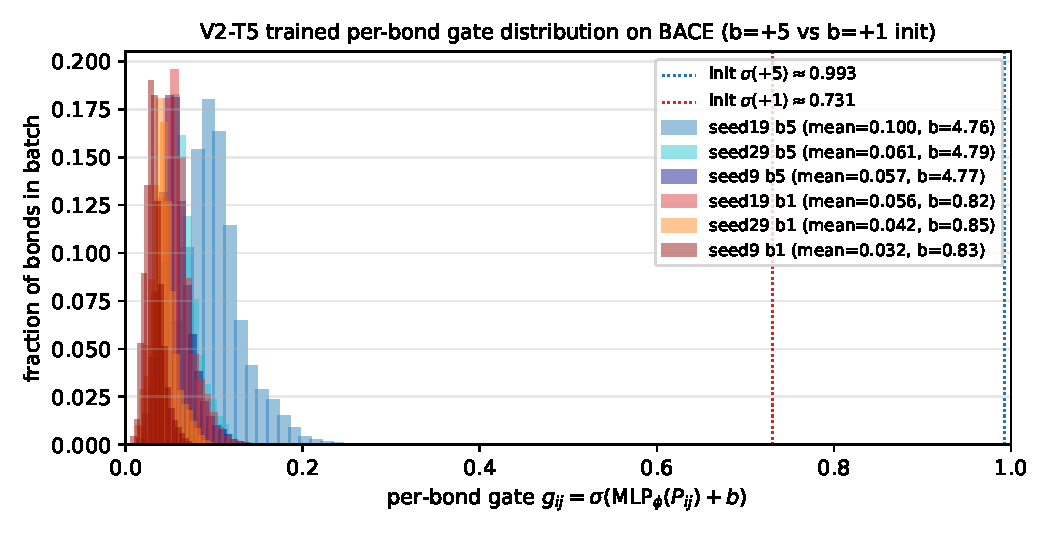
\includegraphics[width=\columnwidth]{figures/gate_distribution_bace_v2t5.pdf}
\caption{Trained per-bond gate distribution for V2-T5 on BACE, across three pretraining seeds and two bias-initialization choices. Blue group: $b{=}{+}5$ initialization ($\sigma(5)\approx 0.993$, the default in the paper). Red group: $b{=}{+}1$ ablation ($\sigma(1)\approx 0.731$). Dotted lines mark the initial gate values for each group. In both groups the bias term barely moves during training (final $b\approx 4.77$ for the $+5$ runs and $b\approx 0.83$ for the $+1$ runs), but the MLP weights learn substantial negative shifts, so the trained gates sit far below the initialization. The $b{=}{+}1$ trajectory converges to an even more sparsified Laplacian (mean $\sigma\approx 0.04$); on BACE it ties the $b{=}{+}5$ default at test time ($0.759 \pm 0.019$ vs.\ $0.763 \pm 0.010$, fingerprint saturated), while on the original three BBBP seeds it drops $3.3$ AUC points and the gate fails to enter the aromatic-routing basin. Source data: the \texttt{mlp\_phi\_stats/} audit JSONs in the artifact.}
\label{fig:gate}
\end{figure}

\section{DFT Gate-Movement Probe}
\subsection{Gate-movement probe: data-bound, not a wiring artifact}
A skeptic could object that T8's co-update gates never trained, so the negative reflects a dead channel rather than an absent signal. We close this loophole with a pre-registered probe. The finetune high-learning-rate gate group originally matched only the attention gate (T7), missing T8's node, pair, and feed-forward gates; we fixed it to train all four and re-ran T8 and its random control on MMFF QM9-$\mu$. The gates now move (per-layer pair gates reach $\sim{\pm}0.3$--$0.4$ from a zero init, node and FFN gates $\sim{\pm}0.1$), so the channel is demonstrably active. But the co-update gets \emph{worse}, not better: gate-fixed T8 RMSE $0.989$ versus the buggy-gate $0.966$, and the apparent geometry effect \emph{collapses} from $-0.033$ to $-0.003$. Under the pre-registered rule---gates move \emph{and} error improves implies a suppressed signal; gates move \emph{without} improvement implies a data-bound limit---this is decisive: the negative is data-bound, not a design or wiring artifact. The small MMFF ``effect'' was a frozen-gate edge-weight side path, not the intended co-update mechanism.

\section{Frozen-Probe-to-Finetune Correction: 2D-only V0 Detail}
\paragraph{The $0.758$ reading does not reproduce.}
Re-running the encoder's own canonical protocol (all-structure pretraining,
frozen V0, but trained to convergence: $\sim$1000 pretrain epochs and a
2000-epoch logistic-regression head) lifts BACE V0 from $0.758$ to
$0.822$ on the same single fold, and a three-split DeepChem scaffold
reproduction (P6) gives $0.823$. The published $0.758$ is therefore an
under-trained-probe artifact: a properly converged frozen V0 sits at
$\sim$0.82 regardless of split, $+0.06$ AUC above the headline weak reading.

\paragraph{Finetuning closes the gap to fingerprints.}
Unfreezing the encoder (40-epoch finetune, gate/encoder/head learning rates
$10^{-2}/10^{-4}/10^{-3}$) lifts V0 further to BACE $0.886$, BBBP $0.860$,
and FreeSolv $0.602$ RMSE. Table~\ref{tab:frozen-vs-finetune} gives the
per-dataset frozen$\to$finetune deltas for V0. Finetuning makes the deep
encoder competitive on the non-saturated subset: properly finetuned, the 2D
V0 encoder is \emph{competitive with} the Random-Forest fingerprint baseline on BACE ($0.886$ vs.\ RF $0.894$--$0.906$ across split protocols) and \emph{beats}
it on BBBP ($0.860$ vs.\ RF $0.799$--$0.814$) and on FreeSolv; these finetune cells are a single fold-0, so the cross-split RF comparison is indicative. The earlier
``$+11$~AUC finetune lift'' over $0.758$ was a cross-protocol artifact of
comparing against the under-trained probe; the real finetune-minus-frozen
delta is $+0.00$ to $+0.10$ and dataset-dependent (BACE all $+0.064$,
BBBP $+0.079$ to $+0.098$, FreeSolv $-0.054$ to $+0.008$ RMSE).

\begin{table}[t]
\centering
\caption{Frozen vs.\ finetuned 2D-only encoder (V0), $n{=}3$ init seeds,
single fold. ``all'' = transductive pretraining (train+valid+test
structures); ``train'' = inductive pretraining (encoder never sees
valid/test). BACE/BBBP are AUC ($\uparrow$); FreeSolv is RMSE
($\downarrow$). $\Delta$ is finetune~$-$~frozen (positive favors finetune
for AUC; for RMSE a negative $\Delta$ favors finetune).
Source: \texttt{inductive\_sweep\_2026-06-01.json},
\texttt{tables.frozen\_vs\_finetune\_V0}.}
\label{tab:frozen-vs-finetune}
\small
\begin{tabular}{llrrr}
\toprule
Dataset & Pretrain & Frozen & Finetune & $\Delta$ \\
\midrule
BACE (AUC)     & all   & 0.822 & 0.886 & $+0.064$ \\
BACE (AUC)     & train & 0.874 & 0.875 & $+0.001$ \\
BBBP (AUC)     & all   & 0.763 & 0.860 & $+0.098$ \\
BBBP (AUC)     & train & 0.785 & 0.864 & $+0.080$ \\
FreeSolv (RMSE)& all   & 0.656 & 0.602 & $-0.054$ \\
FreeSolv (RMSE)& train & 0.658 & 0.666 & $+0.008$ \\
\bottomrule
\end{tabular}
\end{table}

\section{Spectral and Message-Passing GNN Background}
\paragraph{Spectral and message-passing GNNs.}
Spectral GNNs trace back to the Chebyshev formulation of \citet{defferrard2016chebnet}, simplified by \citet{kipf2017gcn}, and complemented by attention-based \texttt{GAT} \citep{velickovic2018gat} and injective \texttt{GIN} \citep{xu2019gin}. A complementary line revisits which polynomial basis yields the most expressive filter: Bernstein with non-negativity \citep{he2021bernnet}, generalized PageRank \citep{chien2021gprgnn}, and Chebyshev~II \citep{he2022chebnetii}, the basis we adopt. An early molecular use of this adaptive-edge-spectral idea is the consistent-edge-attention spectral GCN of \citet{shang2021eagcn}, which lets attention modulate the Laplacian; we follow the same move but route the per-edge weight through a Uni-Mol pair representation. Recently, \citet{chen2024polygcl} extended polynomial filters to graph contrastive learning, and \citet{nogueira2025spectra} used the eigenspectrum for target-aware augmentation. For molecular property prediction itself, \citet{gilmer2017mpnn} unified earlier models under message-passing, and \texttt{AttentiveFP} \citep{xiong2020attentivefp} remains a frequent attention-aggregation baseline; both operate on bond topology only, motivating the through-space gating studied here.
The edge-gated spectral operation itself predates this work: \texttt{EAGCN}
\citep{shang2021eagcn} already lets a learned edge attention modulate the
molecular Laplacian, and \texttt{FAGCN} \citep{bo2021fagcn} introduces the
per-edge scalar gate in $[-1,1]$ that mixes low- and high-pass propagation which
our dual-path gate reuses; we therefore claim \emph{no edge-gating novelty}, only
that the gate values are \emph{sourced from a frozen 3D Uni-Mol pair} and then
\emph{audited}. More broadly, a learned spectral/Chebyshev backbone on molecules
is well established---from \texttt{EAGCN} \citep{shang2021eagcn} through
\texttt{Specformer} \citep{bo2023specformer} and the target-aware spectral
augmentation of \citet{nogueira2025spectra}---so the Chebyshev~II encoder is a
deliberately standard \emph{instrument}; our contribution is the combination of
\emph{frozen-3D-into-spectral} injection with a shape-matched random-pair null
protocol, not the spectral filter.

\section{Three-Dimensional Representations and Self-Supervised Pretraining Background}
\paragraph{Three-dimensional representations and self-supervised pretraining.}
Three-dimensional models inject coordinate information via continuous-filter convolutions \citep{schutt2017schnet} (also the conceptual ancestor of our GBF FreeSolv-side control), directional angles \citep{klicpera2020dimenet}, or $E(n)$ equivariance \citep{satorras2021egnn}; \texttt{Uni-Mol} \citep{zhou2023unimol} pretrains an SE(3)-equivariant encoder and exposes a dense pair tensor $P \in \mathbb{R}^{N\times N\times d_p}$ that we consume frozen, and \texttt{Frad} \citep{feng2024frad} extends 3D pretraining with anisotropic-noise denoising. On the self-supervised side, \texttt{MolCLR} \citep{wang2022molclr}, \texttt{GROVER} \citep{rong2020grover}, and \texttt{GraphMVP} \citep{liu2022graphmvp} cover 2D contrastive, graph-transformer, and 2D--3D alignment; \texttt{GEM} \citep{fang2022gem}, \texttt{3D Infomax} \citep{stark2022infomax}, \texttt{Mole-BERT} \citep{xia2023molebert}, and \texttt{KPGT} \citep{li2023kpgt} progressively add geometry-aware objectives, mutual-information maximization, and RDKit-knowledge fusion. More recent multi-task pretraining at moderate scale (\texttt{MiniMol}, \citealp{klaeser2024minimol}) rivals foundation models on TDC ADMET; on the cheminformatics side, \texttt{MapLight} \citep{notwell2023maplight} and \texttt{NovoExpert}-2 \citep{novoexpert2026} show that fingerprint + gradient-boosted trees top the TDC ADMET leaderboard, reinforcing that a strong fingerprint baseline is harder to beat than the graph-side literature reports. Our work is complementary and deliberately not method-proposing: rather than introduce a new SSL objective or architecture, we audit---under the matched-protocol regime advocated by the \texttt{MoleculeNet} benchmark \citep{wu2018moleculenet}---whether existing downstream-time mechanisms for injecting a frozen 3D pair representation into a 2D spectral backbone improve over strong 2D and classical controls.

\section{Geometry-Pure Stress Test: Motivation}
\subsection{Motivation: is the negative just weak targets or coarse 3D?}
The matched-protocol audit (Sec.~\ref{sec:experiments}) shows a descriptor random forest matching or beating frozen 3D-pair injection on saturated ADMET endpoints. Two confounds could explain that negative without indicting 3D injection itself: the targets may simply not \emph{need} geometry (so any geometry-blind model wins), and the injected coordinates were approximate RDKit-MMFF conformers, which prior work reports can collapse a geometry signal. We therefore run a geometry-pure stress test on quantum targets, sweeping both axes: a target that \emph{is} geometry (the QM9 dipole $\mu$, where a 2D model is information-limited by construction) and a coordinate source that is the gold-standard B3LYP/6-31G(2df,p) DFT geometry, not MMFF. To separate the contribution of the injection \emph{architecture} from the contribution of the \emph{geometry} it carries, every 3D arm is paired with a \texttt{random} control in which the per-molecule Uni-Mol pair representation is shuffled, destroying geometry while preserving capacity and wiring. We define the \emph{geometry effect} as $\mathrm{RMSE}(\text{real}) - \mathrm{RMSE}(\text{random})$: negative means real coordinates help beyond architecture.

\end{document}
